\documentclass[11pt,a4paper]{report}
\usepackage[textwidth=37em,vmargin=30mm]{geometry}
\usepackage{calc,xunicode,amsmath,amssymb,paralist,enumitem,tabu,booktabs,datetime2,xeCJK,xeCJKfntef,listings}
\usepackage{tocloft,fancyhdr,tcolorbox,xcolor,graphicx,eso-pic,xltxtra,xelatexemoji}

\newcommand{\envyear}[0]{2025}
\newcommand{\envdatestr}[0]{2025-09-09}
\newcommand{\envfinaldir}[0]{webdb/2025/20250909/final}

\usepackage[hidelinks]{hyperref}
\hypersetup{
    colorlinks=false,
    pdfpagemode=FullScreen,
    pdftitle={Web Digest - \envdatestr}
}

\setlength{\cftbeforechapskip}{10pt}
\renewcommand{\cftchapfont}{\rmfamily\bfseries\large\raggedright}
\setlength{\cftbeforesecskip}{2pt}
\renewcommand{\cftsecfont}{\sffamily\small\raggedright}

\setdefaultleftmargin{2em}{2em}{1em}{1em}{1em}{1em}

\usepackage{xeCJK,xeCJKfntef}
\xeCJKsetup{PunctStyle=plain,RubberPunctSkip=false,CJKglue=\strut\hskip 0pt plus 0.1em minus 0.05em,CJKecglue=\strut\hskip 0.22em plus 0.2em}
\XeTeXlinebreaklocale "zh"
\XeTeXlinebreakskip = 0pt


\setmainfont{Brygada 1918}
\setromanfont{Brygada 1918}
\setsansfont{IBM Plex Sans}
\setmonofont{JetBrains Mono NL}
\setCJKmainfont{Noto Serif CJK SC}
\setCJKromanfont{Noto Serif CJK SC}
\setCJKsansfont{Noto Sans CJK SC}
\setCJKmonofont{Noto Sans CJK SC}

\setlength{\parindent}{0pt}
\setlength{\parskip}{8pt}
\linespread{1.15}

\lstset{
	basicstyle=\ttfamily\footnotesize,
	numbersep=5pt,
	backgroundcolor=\color{black!5},
	showspaces=false,
	showstringspaces=false,
	showtabs=false,
	tabsize=2,
	captionpos=b,
	breaklines=true,
	breakatwhitespace=true,
	breakautoindent=true,
	linewidth=\textwidth
}






\newcommand{\coverpic}[2]{
    % argv: itemurl, authorname
    Cover photo by #2~~(\href{#1}{#1})
}
\newcommand{\makeheader}[0]{
    \begin{titlepage}
        % \newgeometry{hmargin=15mm,tmargin=21mm,bmargin=12mm}
        \begin{center}
            
            \rmfamily\scshape
            \fontspec{BaskervilleF}
            \fontspec{Old Standard}
            \fontsize{59pt}{70pt}\selectfont
            WEB\hfill DIGEST
            
            \vfill
            % \vskip 30pt
            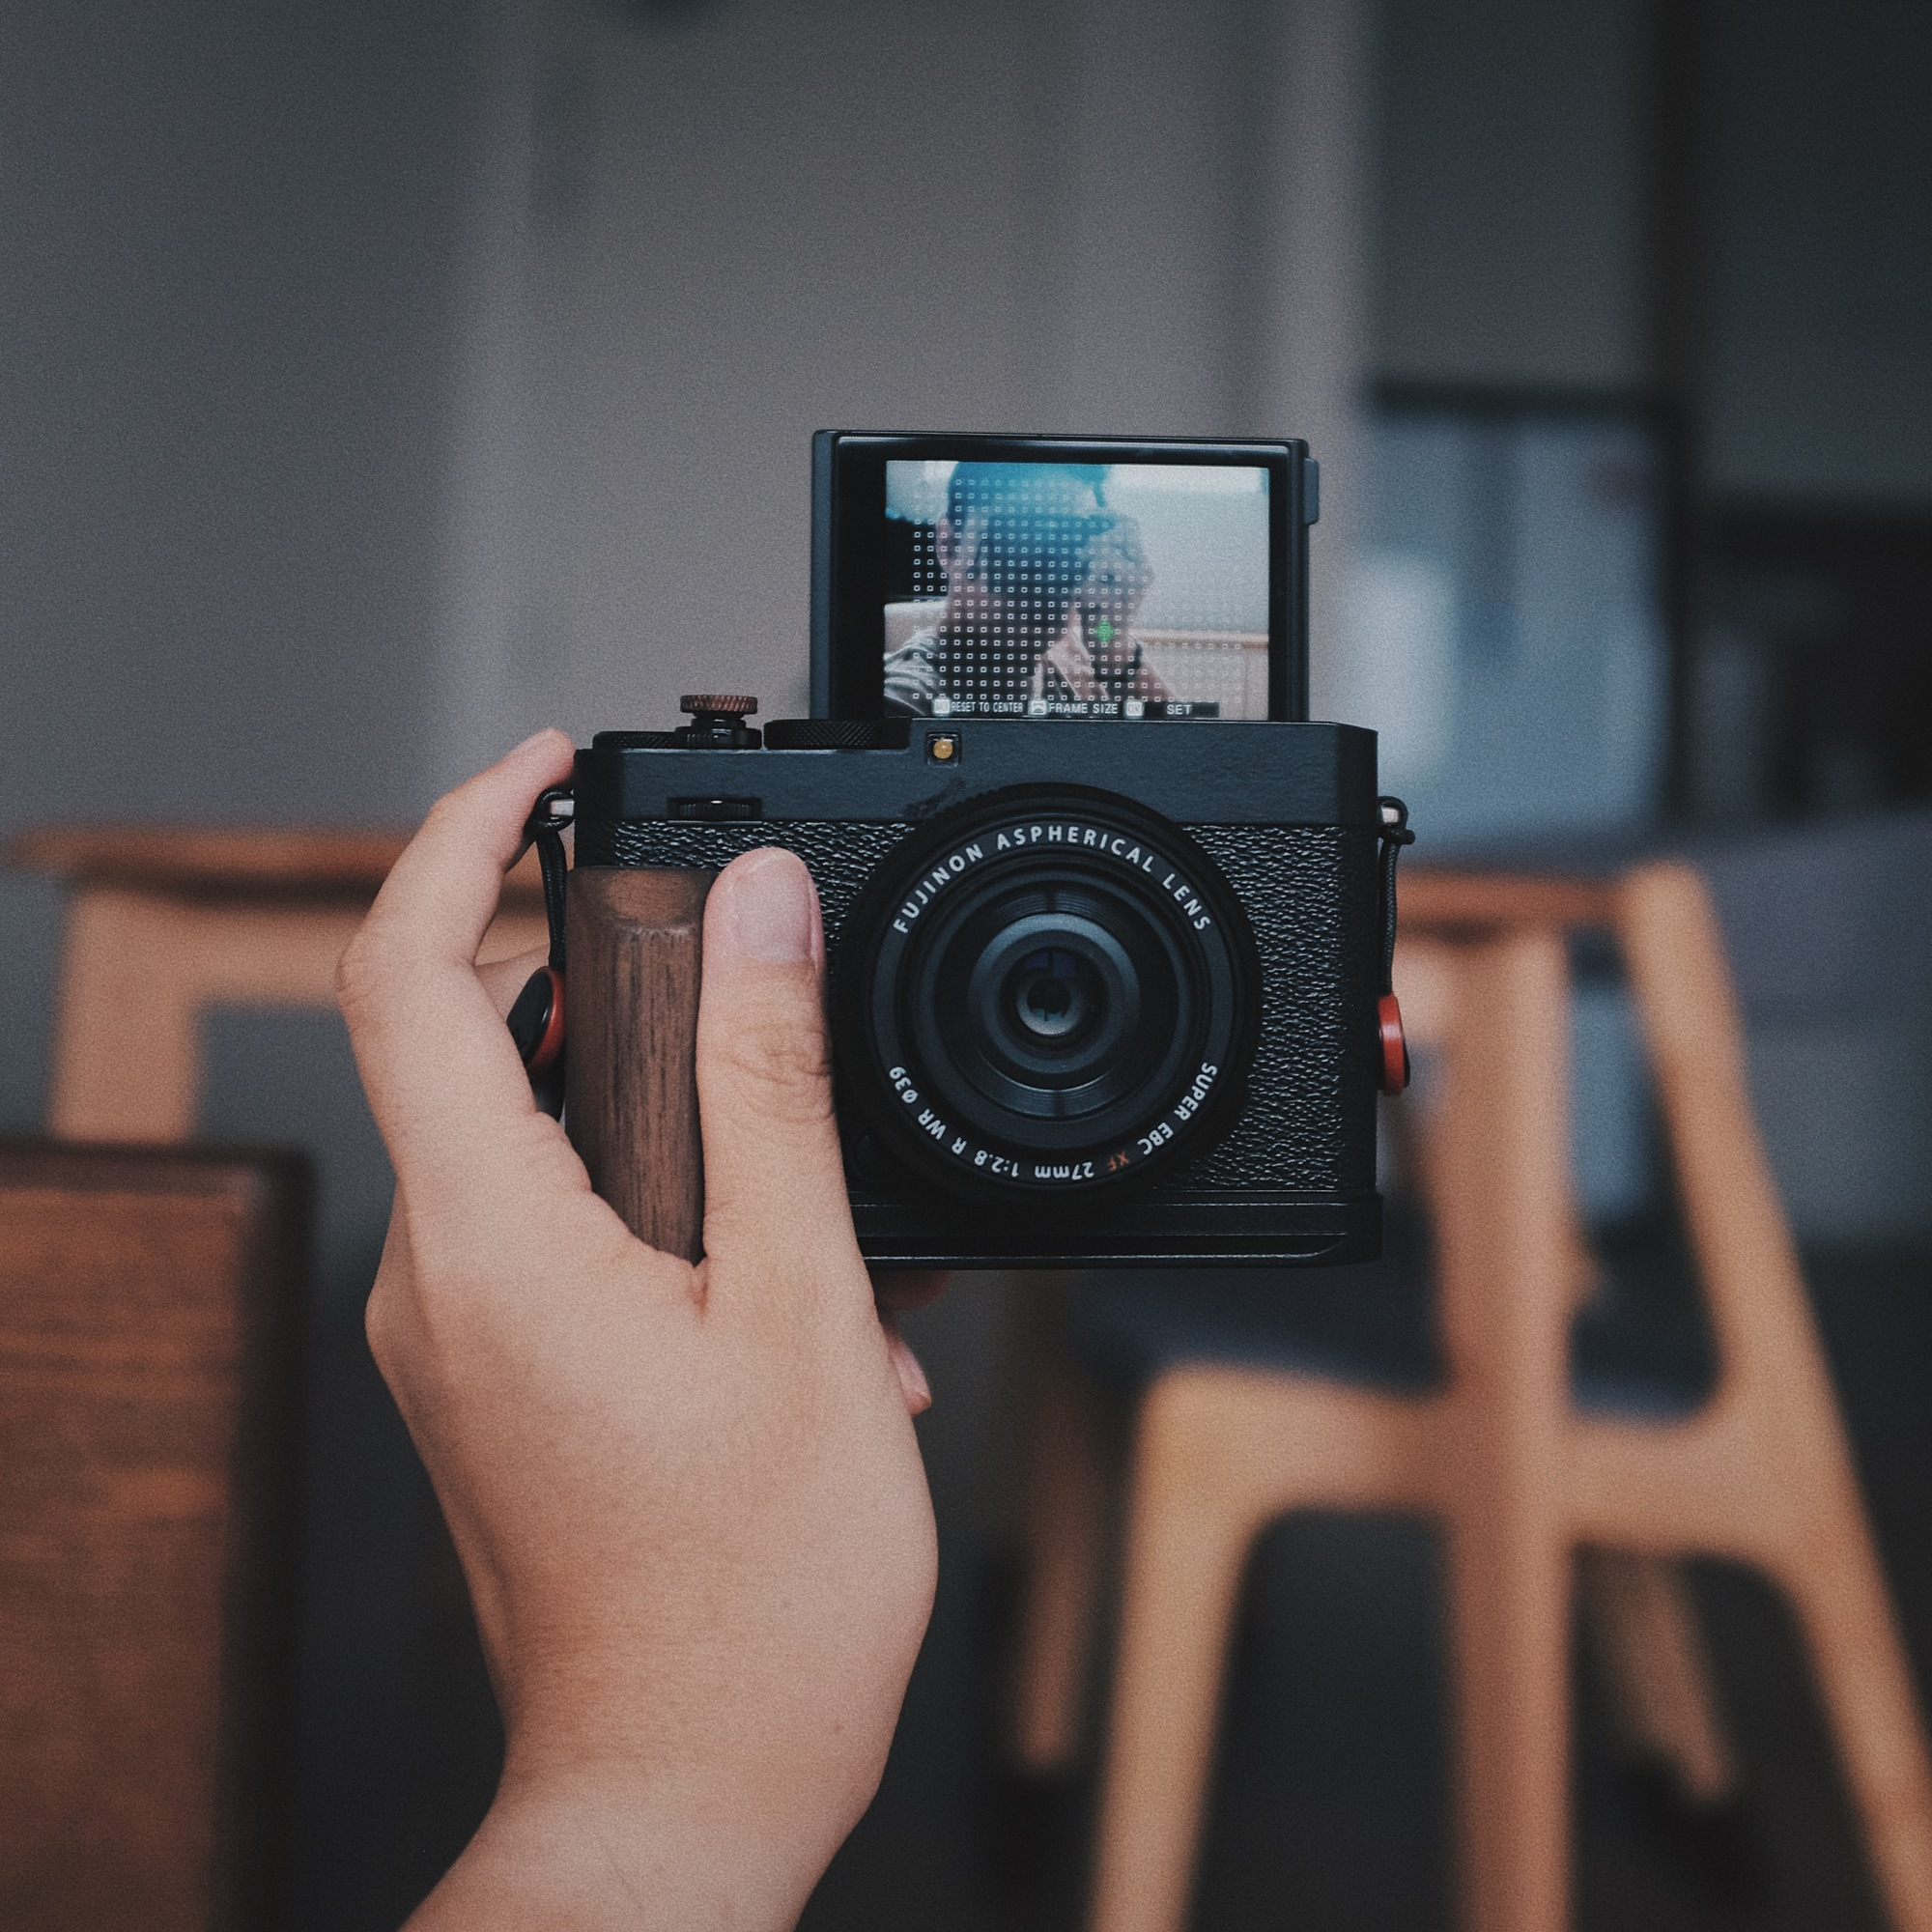
\includegraphics[width=\linewidth]{\envfinaldir/coverpic-prod.jpg}\par
            % \vskip 30pt
            \vfill

            \normalsize\rmfamily\scshape
            \copyright{} The Web Digest Project \hfill\large \envdatestr
        \end{center}
    \end{titlepage}
    % \restoregeometry
}
\newcommand{\simplehref}[1]{%
    \textcolor{blue!80!green}{\href{#1}{#1}}%
}
\renewcommand{\contentsname}{\center\Huge\sffamily\bfseries Contents\par\vskip 20pt}
\newcounter{ipartcounter}
\setcounter{ipartcounter}{0}
\newcommand{\ipart}[1]{
    % \vskip 20pt
    \clearpage
    \stepcounter{ipartcounter}
    \phantomsection
    \addcontentsline{toc}{chapter}{#1}
    % \begin{center}
    %     \Huge
    %     \sffamily\bfseries
    %     #1
    % \end{center}
    % \vskip 20pt plus 7pt
}
\newcounter{ichaptercounter}
\setcounter{ichaptercounter}{0}
\newcommand{\ichapter}[1]{
    % \vskip 20pt
    \clearpage
    \stepcounter{ichaptercounter}
    \phantomsection
    \addcontentsline{toc}{section}{\numberline{\arabic{ichaptercounter}}#1}
    \begin{center}
        \Huge
        \sffamily\bfseries
        #1
    \end{center}
    \vskip 20pt plus 7pt
}
\newcommand{\entrytitlefont}[1]{\subsection*{\raggedright\Large\sffamily\bfseries#1}}
\newcommand{\entryitemGeneric}[2]{
    % argv: title, url
    \parbox{\linewidth}{
        \entrytitlefont{#1}\par\vskip 5pt
        \footnotesize\ttfamily\mdseries
        \simplehref{#2}
    }\vskip 11pt plus 11pt minus 1pt
}
\newcommand{\entryitemGithub}[3]{
    % argv: title, url, desc
    \parbox{\linewidth}{
        \entrytitlefont{#1}\par\vskip 5pt
        \footnotesize\ttfamily\mdseries
        \simplehref{#2}\par\vskip 5pt
        \small\rmfamily\mdseries#3
    }\vskip 11pt plus 11pt minus 1pt
}
\newcommand{\entryitemAp}[3]{
    % argv: title, url, desc
    \parbox{\linewidth}{
        \entrytitlefont{#1}\par\vskip 5pt
        \footnotesize\ttfamily\mdseries
        \simplehref{#2}\par\vskip 5pt
        \small\rmfamily\mdseries#3
    }\vskip 11pt plus 11pt minus 1pt
}
\newcommand{\entryitemHackernews}[3]{
    % argv: title, hnurl, rawurl
    % \parbox{\linewidth}{
    %     \entrytitlefont{#1}\par\vskip 5pt
    %     \footnotesize\ttfamily\mdseries
    %     \simplehref{#3}\par
    %     \textcolor{black!50}{\href{#2}{#2}}
    % }\vskip 11pt plus 11pt minus 1pt
    \begin{minipage}{\linewidth}
            \entrytitlefont{#1}\par\vskip 5pt
            \footnotesize\ttfamily\mdseries
            \simplehref{#3}\par
            \textcolor{black!50}{\href{#2}{#2}}
    \end{minipage}\par\vskip 11pt plus 11pt minus 1pt
}







\begin{document}

\makeheader

\tableofcontents\clearpage




\ipart{Developers}
\ichapter{Hacker News}
\entryitemTwoLinks{Ex-WhatsApp cybersecurity head says Meta endangered billions of users}{https://news.ycombinator.com/item?id=45174221}{https://www.theguardian.com/technology/2025/sep/08/meta-user-data-lawsuit-whatsapp}

\entryitemTwoLinks{YouTube views are down (don't panic)}{https://news.ycombinator.com/item?id=45173455}{https://www.jeffgeerling.com/blog/2025/youtube-views-are-down-dont-panic}

\entryitemTwoLinks{Chat Control Must Be Stopped}{https://news.ycombinator.com/item?id=45173277}{https://www.privacyguides.org/articles/2025/09/08/chat-control-must-be-stopped/}

\entryitemTwoLinks{iPhone dumbphone}{https://news.ycombinator.com/item?id=45171200}{https://stopa.io/post/297}

\entryitemTwoLinks{Signal Secure Backups}{https://news.ycombinator.com/item?id=45170515}{https://signal.org/blog/introducing-secure-backups/}

\entryitemTwoLinks{OpenWrt: A Linux OS targeting embedded devices}{https://news.ycombinator.com/item?id=45170087}{https://openwrt.org/}

\entryitemTwoLinks{Job mismatch and early career success}{https://news.ycombinator.com/item?id=45169892}{https://www.nber.org/papers/w34215}

\entryitemTwoLinks{NPM debug and chalk packages compromised}{https://news.ycombinator.com/item?id=45169657}{https://www.aikido.dev/blog/npm-debug-and-chalk-packages-compromised}

\entryitemTwoLinks{Will Amazon S3 Vectors kill vector databases or save them?}{https://news.ycombinator.com/item?id=45169624}{https://zilliz.com/blog/will-amazon-s3-vectors-kill-vector-databases-or-save-them}

\entryitemTwoLinks{Google gets away almost scot-free in US search antitrust case}{https://news.ycombinator.com/item?id=45169584}{https://www.computerworld.com/article/4052428/google-gets-away-almost-scot-free-in-us-search-antitrust-case.html}

\entryitemTwoLinks{Clankers Die on Christmas}{https://news.ycombinator.com/item?id=45169275}{https://remyhax.xyz/posts/clankers-die-on-christmas/}

\entryitemTwoLinks{Dietary omega-3 polyunsaturated fatty acids as a protective factor of myopia}{https://news.ycombinator.com/item?id=45169157}{https://bjo.bmj.com/content/early/2025/08/17/bjo-2024-326872}

\entryitemTwoLinks{Experimenting with Local LLMs on macOS}{https://news.ycombinator.com/item?id=45168953}{https://blog.6nok.org/experimenting-with-local-llms-on-macos/}

\entryitemTwoLinks{Meta suppressed research on child safety, employees say}{https://news.ycombinator.com/item?id=45167705}{https://www.washingtonpost.com/investigations/2025/09/08/meta-research-child-safety-virtual-reality/}

\entryitemTwoLinks{AI might yet follow the path of previous technological revolutions}{https://news.ycombinator.com/item?id=45167625}{https://www.economist.com/finance-and-economics/2025/09/04/what-if-artificial-intelligence-is-just-a-normal-technology}

\entryitemTwoLinks{ICEBlock handled my vulnerability report in the worst possible way}{https://news.ycombinator.com/item?id=45167534}{https://micahflee.com/iceblock-handled-my-vulnerability-report-in-the-worst-possible-way/}

\entryitemTwoLinks{A clickable visual guide to the Rust type system}{https://news.ycombinator.com/item?id=45167401}{https://rustcurious.com/elements/}

\entryitemTwoLinks{Indiana Jones and the Last Crusade Adventure Prototype Recovered for the C64}{https://news.ycombinator.com/item?id=45167245}{https://www.gamesthatwerent.com/2025/09/indiana-jones-and-the-last-crusade-adventure-prototype-recovered-for-the-commodore-64/}

\entryitemTwoLinks{VMware's in court again. Customer relationships rarely go this wrong}{https://news.ycombinator.com/item?id=45167239}{https://www.theregister.com/2025/09/08/vmware\_in\_court\_opinion/}

\entryitemTwoLinks{14 Killed in anti-government protests in Nepal}{https://news.ycombinator.com/item?id=45166972}{https://www.tribuneindia.com/news/world/massive-protests-in-nepal-over-social-media-ban/}\ichapter{Phoronix}
\entryitemGeneric{\hskip 0pt{}New Linux Patches Enhance Intel Nested Virtualization Performance On Linux}{https://www.phoronix.com/news/Linux-KVM-Nested-Intel-VMX-Perf}

\entryitemGeneric{\hskip 0pt{}First Benchmarks Of Windows 11 25H2 vs. Ubuntu 25.10 On AMD Ryzen 9 9950X}{https://www.phoronix.com/review/windows-11-25h2-ubuntu-2510}

\entryitemGeneric{\hskip 0pt{}KDE Plasma 6 On Wayland Can Work Fine On FreeBSD}{https://www.phoronix.com/news/FreeBSD-KDE-Plasma-Wayland}

\entryitemGeneric{\hskip 0pt{}Linux 6.18 To Introduce Support For Next-Gen eUSB2V2 Web Cameras}{https://www.phoronix.com/news/Linux-6.18-eUSB2V2-Web-Cams}

\entryitemGeneric{\hskip 0pt{}XFS File-System Ready To Enable Online Fsck Support By Default}{https://www.phoronix.com/news/XFS-Ready-Online-FSCK-Default}

\entryitemGeneric{\hskip 0pt{}Linux Looks Ready To Introduce "Sheaves" For Opt-In Per-CPU Array-Based Caching Layer}{https://www.phoronix.com/news/Linux-6.18-Likely-Sheaves}

\entryitemGeneric{\hskip 0pt{}AMD-Xilinx Versal TRNG Driver Queued Ahead Of Linux 6.18}{https://www.phoronix.com/news/AMD-Xilinx-Versal-TRNG-Driver}

\entryitemGeneric{\hskip 0pt{}Linux 6.17-rc5 Released With NVIDIA "Nouveau" Driver Stability Issues Addressed}{https://www.phoronix.com/news/Linux-6.17-rc5}

\entryitemGeneric{\hskip 0pt{}Intel Preps Wildcat Lake Display Support For Linux 6.18, "enable\_panel\_replay" Option}{https://www.phoronix.com/news/Intel-DRM-Next-Linux-6.18}


\ipart{Developers~~~~(zh-Hans)}
\ichapter{Solidot}
\entryitemGeneric{\hskip 0pt{}Firefox ESR 115 将支持到 2026 年 3 月}{https://www.solidot.org/story?sid=82246}

\entryitemGeneric{\hskip 0pt{}Windows 第三方工具允许用户禁用所有 AI 功能}{https://www.solidot.org/story?sid=82245}

\entryitemGeneric{\hskip 0pt{}类似人类,每棵树都有独一无二的微生物组}{https://www.solidot.org/story?sid=82244}

\entryitemGeneric{\hskip 0pt{}特斯拉改变了 Full Self-Driving 的意义,放弃承诺自动驾驶}{https://www.solidot.org/story?sid=82243}

\entryitemGeneric{\hskip 0pt{}美国计划限制进口中国无人机}{https://www.solidot.org/story?sid=82242}

\entryitemGeneric{\hskip 0pt{}Anthropic 向图书作者支付 15 亿美元和解侵权诉讼}{https://www.solidot.org/story?sid=82241}

\entryitemGeneric{\hskip 0pt{}Firefox 将于 2026 年 9 月停止支持 32 位 Linux 系统}{https://www.solidot.org/story?sid=82240}

\entryitemGeneric{\hskip 0pt{}Google 因广告技术业务的反垄断行为被欧盟罚款 34.5 亿美元 }{https://www.solidot.org/story?sid=82239}

\entryitemGeneric{\hskip 0pt{}英国政府试用 M365 Copilot 后未发现明显的生产力提升}{https://www.solidot.org/story?sid=82238}\ichapter{V2EX}
\entryitemGeneric{\hskip 0pt{}[分享创造] 0dMIPS: MIPS64 ISA 硬件部分实现}{https://www.v2ex.com/t/1157901}

\entryitemGeneric{\hskip 0pt{}[信息安全] 登录接口明文密码在浏览器端先加盐 SHA512 一次,服务端再用 bcrypt 等慢哈希算法二次加密存储是最佳实践吗?为什么多个大厂都发生过不小心在日志输出用户明文密码的事件,不加密或可逆加密传输用户密码仍是主流}{https://www.v2ex.com/t/1157900}

\entryitemGeneric{\hskip 0pt{}[Apple] Time Machine 备份如何上云?}{https://www.v2ex.com/t/1157899}

\entryitemGeneric{\hskip 0pt{}[微信] 企业微信,就可以为所欲为了?}{https://www.v2ex.com/t/1157898}

\entryitemGeneric{\hskip 0pt{}[问与答] 如何及时收到可以抢票演唱会的通知?}{https://www.v2ex.com/t/1157897}

\entryitemGeneric{\hskip 0pt{}[问与答] 你一定没有梦到过手机}{https://www.v2ex.com/t/1157896}

\entryitemGeneric{\hskip 0pt{}[分享创造] 快点装机——一个装机导航网站,提供装机模拟、系统下载、软件下载等一站式服务。}{https://www.v2ex.com/t/1157895}

\entryitemGeneric{\hskip 0pt{}[硬件] 家里用了 7 年的吸顶 AP 时好时坏,想换个能带客户端隔离的吸顶 AP,预算 800 左右,求推荐?}{https://www.v2ex.com/t/1157894}

\entryitemGeneric{\hskip 0pt{}[分享发现] 找到个 Nano Banana 薅羊毛的免费使用入口}{https://www.v2ex.com/t/1157893}

\entryitemGeneric{\hskip 0pt{}[问与答] 工行新开户有啥信用卡推荐吗?}{https://www.v2ex.com/t/1157892}

\entryitemGeneric{\hskip 0pt{}[问与答] 小米王腾被撸了??}{https://www.v2ex.com/t/1157891}

\entryitemGeneric{\hskip 0pt{}[职场话题] 请问有哪些便宜的期刊,聘职称用}{https://www.v2ex.com/t/1157890}

\entryitemGeneric{\hskip 0pt{}[问与答] 百万医疗保险, 0 起付线,无条件续保。这样的有吗?}{https://www.v2ex.com/t/1157889}

\entryitemGeneric{\hskip 0pt{}[分享创造] 做了个歌词评价工具,有兴趣的朋友们可以试用下给下反馈呀}{https://www.v2ex.com/t/1157888}

\entryitemGeneric{\hskip 0pt{}[职场话题] 小红书交易搜索算法怎么样?}{https://www.v2ex.com/t/1157887}

\entryitemGeneric{\hskip 0pt{}[问与答] 兄弟们 跪求 有用的灭蟑螂药~~}{https://www.v2ex.com/t/1157884}

\entryitemGeneric{\hskip 0pt{}[问与答] 硬盘盘符丢失,我该怎么办,求搭救。}{https://www.v2ex.com/t/1157883}

\entryitemGeneric{\hskip 0pt{}[程序员] 求地图 beijing.osm.pbf 数据}{https://www.v2ex.com/t/1157882}

\entryitemGeneric{\hskip 0pt{}[分享创造] 一个无需安装、无需注册的 HEIC → JPG 在线转换小工具}{https://www.v2ex.com/t/1157881}

\entryitemGeneric{\hskip 0pt{}[问与答] 大家做梦的时候会经常梦到家人吗?}{https://www.v2ex.com/t/1157880}

\entryitemGeneric{\hskip 0pt{}[分享创造] 分享一个通用的 VSCode I18n 插件,适合有复杂国际化需求或技术栈特殊的项目}{https://www.v2ex.com/t/1157877}

\entryitemGeneric{\hskip 0pt{}[程序员] 使用招行 VISA 卡购买 IDEA 付款被拒}{https://www.v2ex.com/t/1157875}

\entryitemGeneric{\hskip 0pt{}[程序员] 最近有什么随身 WIFI 推荐吗}{https://www.v2ex.com/t/1157874}

\entryitemGeneric{\hskip 0pt{}[VPS] 老哥们咨询一下: ClawCloud 的 VPS 如何 今年黑五有年付的机器么~~}{https://www.v2ex.com/t/1157873}

\entryitemGeneric{\hskip 0pt{}[iOS] AI 辅助编程实战:从零到一开发 Swift 性能框架的经验分享}{https://www.v2ex.com/t/1157872}

\entryitemGeneric{\hskip 0pt{}[问与答] Win11 下 Telegram Desktop 无法启动}{https://www.v2ex.com/t/1157870}

\entryitemGeneric{\hskip 0pt{}[酷工作] [招聘] Golang/Rust 开发工程师}{https://www.v2ex.com/t/1157869}

\entryitemGeneric{\hskip 0pt{}[分享创造] 做了个 Claude Code 中文文档站:快速开始 / 故障排查 / 模板库(持续更新)}{https://www.v2ex.com/t/1157868}

\entryitemGeneric{\hskip 0pt{}[Figma] 代验证 figma 教育版本一年}{https://www.v2ex.com/t/1157867}

\entryitemGeneric{\hskip 0pt{}[问与答] 一个小项目,求推荐类似的源码}{https://www.v2ex.com/t/1157866}

\entryitemGeneric{\hskip 0pt{}[问与答] 没卖完的期房会怎么处理? 12 月交付的房子,是现在买,还是交付后再买?}{https://www.v2ex.com/t/1157865}

\entryitemGeneric{\hskip 0pt{}[问与答] 2025 年已过 2/3,大盘已迈过 3800 点,截至目前,今年你的股票/期货或者其他权益资产收益怎么样}{https://www.v2ex.com/t/1157864}

\entryitemGeneric{\hskip 0pt{}[推广] 我又做了个小玩意: 定年投资计算器}{https://www.v2ex.com/t/1157863}

\entryitemGeneric{\hskip 0pt{}[问与答] 有没有根据 PNG 或者 JPG 在线生成 3D 文件的 AI?}{https://www.v2ex.com/t/1157862}

\entryitemGeneric{\hskip 0pt{}[分享创造] 诗序:玩游戏的方式来背诗}{https://www.v2ex.com/t/1157861}

\entryitemGeneric{\hskip 0pt{}[程序员] 上海小办公室转租}{https://www.v2ex.com/t/1157860}

\entryitemGeneric{\hskip 0pt{}[奇思妙想] 对稳定币支付的一种设想}{https://www.v2ex.com/t/1157859}

\entryitemGeneric{\hskip 0pt{}[Apple] 国行苹果 AI 预计将在年底上线, iOS 26.1 或 26.2,与阿里和百度合作,阿里将充当审核引擎角色,百度将充当主要模型(在线)角色。}{https://www.v2ex.com/t/1157855}

\entryitemGeneric{\hskip 0pt{}[问与答] 想搞个二手安卓手机用于开发,有没有哪个型号比较便宜而且性能还过得去的}{https://www.v2ex.com/t/1157854}

\entryitemGeneric{\hskip 0pt{}[问与答] Google cloud 有工单支持或者群吗?}{https://www.v2ex.com/t/1157853}

\entryitemGeneric{\hskip 0pt{}[VPS] claw vps,遇到非常古怪的问题}{https://www.v2ex.com/t/1157852}

\entryitemGeneric{\hskip 0pt{}[分享发现] 给大家推荐我开发的简历编辑工具}{https://www.v2ex.com/t/1157851}

\entryitemGeneric{\hskip 0pt{}[生活] 爱回收的 Apple Watch 细微划痕实际中怎么判定的}{https://www.v2ex.com/t/1157850}

\entryitemGeneric{\hskip 0pt{}[酷工作] 高德北京-前后端、ai 大模型算法应用都要}{https://www.v2ex.com/t/1157849}

\entryitemGeneric{\hskip 0pt{}[程序员] 表格生图}{https://www.v2ex.com/t/1157848}

\entryitemGeneric{\hskip 0pt{}[问与答] 如何禁止 betterdisplay 检测更新}{https://www.v2ex.com/t/1157847}

\entryitemGeneric{\hskip 0pt{}[生活] 朋友们,请问有江浙沪地区想养小狗的吗?免费送。}{https://www.v2ex.com/t/1157846}

\entryitemGeneric{\hskip 0pt{}[生活] 遇到这样的孩子怎么办?}{https://www.v2ex.com/t/1157845}

\entryitemGeneric{\hskip 0pt{}[NAS] 有没有老哥用 畅网 x86-p6 n150 做 nas 机器}{https://www.v2ex.com/t/1157844}

\entryitemGeneric{\hskip 0pt{}[问与答] 国内大带宽服务器推荐}{https://www.v2ex.com/t/1157842}


\ipart{Generic News}







\clearpage
\leavevmode\vfill
\footnotesize

Copyright \copyright{} 2023-2025 Neruthes and other contributors.

This document is published with CC BY-NC-ND 4.0 license.

The entries listed in this newsletter may be copyrighted by their respective creators.

This newsletter is generated by the Web Digest project.

The newsletters are also delivered via Telegram channel \CJKunderline{\href{https://t.me/webdigestchannel}{https://t.me/webdigestchannel}}.\\
RSS feed is available at \CJKunderline{\href{https://webdigest.pages.dev/rss.xml}{https://webdigest.pages.dev/rss.xml}}.

This newsletter is available in PDF at
\CJKunderline{\href{https://webdigest.pages.dev/}{https://webdigest.pages.dev/}}.

The source code being used to generate this newsletter is available at\\
\CJKunderline{\href{https://github.com/neruthes/webdigest}{https://github.com/neruthes/webdigest}}.

This newsletter is also available in
\CJKunderline{\href{http://webdigest.pages.dev/readhtml/\envyear/WebDigest-20250909.html}{HTML}} and
\CJKunderline{\href{https://github.com/neruthes/webdigest/blob/master/markdown/\envyear/WebDigest-20250909.md}{Markdown}}.


\coverpic{https://unsplash.com/photos/a-tree-grows-on-a-log-in-the-water-qNY60EkL3nE}{Zetong Li}


\end{document}
